\documentclass[prb,12pt]{revtex4-2}

\usepackage{amsmath, amssymb,physics,amsfonts,amsthm}
\usepackage{enumitem}
\usepackage[most]{tcolorbox}
\usepackage{cancel}
\usepackage{booktabs}
\usepackage{tikz}
\usepackage{hyperref}
\usepackage{enumitem}
\usepackage{transparent}
\usepackage{float}
\usepackage{multirow}
\usepackage{subcaption}
\newtheorem{Theorem}{Theorem}
\newtheorem{Proposition}{Theorem}
\newtheorem{Lemma}[Theorem]{Lemma}
\newtheorem{Corollary}[Theorem]{Corollary}
\newtheorem{Example}[Theorem]{Example}
\newtheorem{Remark}[Theorem]{Remark}
\theoremstyle{definition}
\newtheorem{Problem}{Problem}
\theoremstyle{definition}
\newtheorem{Definition}[Theorem]{Definition}
\newenvironment{parts}{\begin{enumerate}[label=(\alph*)]}{\end{enumerate}}
%tikz	
\tcbset{breakable=true,toprule at break = 0mm,bottomrule at break = 0mm}
\usetikzlibrary{patterns}
\usepackage{pgfplots}
\pgfplotsset{compat=1.18}
% definitions of number sets
\newcommand{\N}{\mathbb{N}}
\newcommand{\R}{\mathbb{R}}
\newcommand{\Z}{\mathbb{Z}}
\newcommand{\Q}{\mathbb{Q}}
\newcommand{\C}{\mathbb{C}}
\allowdisplaybreaks
\begin{document}
	\title{Analysis 2 Hausaufgabenblatt Nr. 10}
	\author{Jun Wei Tan}
	\email{jun-wei.tan@stud-mail.uni-wuerzburg.de}
	\affiliation{Julius-Maximilians-Universit\"{a}t W\"{u}rzburg}
	\author{Jonas Hack}
	\affiliation{Julius-Maximilians-Universit\"{a}t W\"{u}rzburg}
	\date{\today}
	\maketitle
%\begin{Problem}
	\begin{parts}
		\item Geben Sie die Definitionen von Gradient, Rotation und Divergenz an.
		\item Wir schreiben die Komponenten des dreidimensionalen Vektorprodukts als
			\[
				(\vec{a}\times \vec{b})_i=\sum_{j,k=1}^3 \epsilon_{ijk}a_jb_k,\] 
				wobei $\epsilon_{ijk}$ der total antisymmetrische Tensor f\"{u}r $\R^3$ ist, mit $\epsilon_{ijk}=1$. Zeigen Sie, dass gilt:
				\begin{align*}
					\sum_{i=1}^3 \epsilon_{ijk}\epsilon_{ilm}=&\delta_{jl}\delta_{km}-\delta_{jm}\delta_{kl}\\
					\frac{1}{2}\sum_{i,j=1}^3 \epsilon_{ijk}\epsilon_{jl}\delta_{kl},
				\end{align*}
				mit $\delta$ dem Kronecker-$\delta$.
			\item Zeigen Sie mit den Formeln aus (b) die folgenden Identitäten für beliebige Vektorfelder $\vec{a},~\vec{b},~\vec{c},~\vec{d}$:
				\begin{align*}
					\vec{a}\cdot(\vec{b}\times\vec{c})&=\vec{b}\cdot (\vec{c}\times \vec{a})=\vec{c}\cdot (\vec{a}\times \vec{b})\\
					\vec{a}\times(\vec{b}\times\vec{c})=&(\vec{a}\cdot\vec{c})\vec{b}-(\vec{a}\cdot\vec{b})\vec{c},\\
					(\vec{a}\times\vec{b})\cdot(\vec{c}\times\vec{d})=*(\vec{a}\cdot\vec{c})(\vec{b}\cdot\vec{d})-(\vec{a}\cdot\vec{d})(\vec{b}\cdot\vec{c})
				\end{align*}
			\item Zeigen Sie damit, dass f\"{u}r beliebige skalare Funktionen $F(\vec{x})$ und Vektorfelder $\vec{A}(\vec{x})$ gilt:
				\begin{align*}
					\curl{\grad{F}}=&0\\
					\div{(\curl{A})}=&0\\
					\curl{\curl{A}}=&\grad{(\div{A})}-\laplacian{A}\\
					\div{(F\vec{A})}=(\grad{F})\cdot\vec{A}+F\div{\vec{A}},
				\end{align*}
				mit $\Delta$ dem Laplace-Operator.
	\end{parts}
\end{Problem} 
\begin{proof}
	\begin{parts}
	\item 
		\begin{align*}
			\text{grad }F=\sum_{i=1}^3 \pdv{F}{x_i}\hat{x}_i\\
			\text{div }\vec{F}=\sum_{i=1}^3 \pdv{F_i}{x_i}\\
			\text{curl }\vec{F}=&\ldots
		\end{align*}
	\item Offensichtlich muss $j\neq k$ und $l\neq m$ sein, ansonsten wäre 1
	\end{parts}
\end{proof}
\begin{Problem}
	
\end{Problem}

%\begin{Problem}
	Betrachten Sie die folgenden Familien von Kraftfeldern auf geeigneten Definitionsbereichen $D_\eta^{(n)}  \subseteq \R^3$
	\begin{align*}
		F_\eta^{(1)}:& D_\eta^{(1)}\ni \va x\to r^\eta\cdot \va x\in \R^3\\
		F_\eta^{(2)}:& D_\eta^{(2)}\ni\va x \to r_{12}^\eta\cdot(x_1\va e_1-x_2\va e_2)\in \R^3\\
		F_\eta^{(3)}:& D_\eta^{(3)}\ni \va x\to r_{12}^\eta\cdot\left( x_2\va e_1-x_1\va e_2 \right) \in\R^3\\
		F_\eta^{(4)}:&D_\eta^{(3)}\ni \va x\to r_{12}^\eta\cdot\left( x_2\va e_1+x_1\va e_2 \right) \in \R^3
	\end{align*}
	wobei $r_{12}=\sqrt{x_1^2+x_2^2} $ und $r=\sqrt{x_1^2+x_2^2+x_3^3} $
	Skizzieren Sie die Felder $\va F_\eta^{(n)}$ als Vektorpfeile in der von den Einheitsvektoren $\va e_1$ und $\va e_2$ aufgespannten Ebene (hier genügt es, zwischen den Fällen $\eta > -1, \eta = -1$ und $\eta < -1$ zu unterscheiden). 
	
	Bestimmen Sie, abhängig von der Potenz $\eta \in \R$,
	\begin{enumerate}
		\item den maximalen Definitionsbereich $D_\eta^{(n)}$,
		\item die maximale Bereiche $C_\eta^{(n)}\subseteq D_\eta^{(n)}$, auf denen $F_\eta^{(n)}$ konservativ ist,
		\item eine Potentialfunktion $V_\eta^{(n)}:C_{\eta}^{(n)}\to \R$ mit $F_\eta^{(n)}=-\grad{V_\eta^{(n)}}$, sofern sie existiert,
		\item das Kurvenintegral
		\[I_\eta^{(n)}(R)=\int_{\gamma_R}\dd{\va\xi}\cdot\va F_\eta^{(n)}(\va\xi)\]
		über den gegen den Uhrzeigersinn umlaufenen Kreis $\gamma_R$ mit Radius $R$ und Mittelpunkt $\va0$ in der von $\va e_1$ und $\va e_2$ aufgespannten Ebene
		\begin{center}
			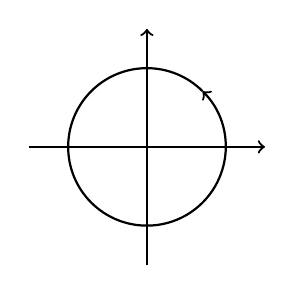
\begin{tikzpicture}
				\draw[thick, ->] (-1.5,0) -- (1.5,0);
				\draw[thick, ->] (0,-1.5) -- (0,1.5);
				\draw[thick, ->] ({1/sqrt(2)},{1/sqrt(2)}) arc (45:405:1);
			\end{tikzpicture}
		\end{center}
	\end{enumerate}
\end{Problem}

%	\begin{Problem}
	Let $V$ be a $\mathbb{K}$-valued vector space. A seminorm on $V$ is a homogeneous map $p:V\to [0,\infty)$ satisfying the triangle inequality, i.e.
	\[
	p(v+w)\le p(v)+p(w)
\]
and
\[
p(\lambda v)=|\lambda|p(v)
\]
for any two vectors $v,w\in V$ and every scalar $\lambda\in\mathbb{K}$.
\begin{parts}
	\item Show that the kernel of a seminorm $p$ is a subspace of $V$.

		Given a seminorm $p$, we say that two vectors $v,w\in V$ are equivalent if there is a vector $u\in \text{ker }p$ such that $w=v+u$. Make yourself clear that this yields an equivalence relation on $V$.
	\item Show that the quotient space $V / \text{ker }p:=V / \sim$ carries a canonical linear structure.
	\item Show that the map
		\[
			\overline{p}:V / \text{ker }p\ni [v]\mapsto p(v)
		\]
		yields a well-defined norm on the quotient space.
\end{parts}
\end{Problem}
\begin{proof}
	\begin{parts}
	\item Clear by definition
	\item Also clear
	\end{parts}
\end{proof}
\begin{Problem}\label{pr:funcanalblatt3-2}
	Let $M$ be a topological space. Show that the space $(\mathcal{C}_b(M), \|\cdot\|_\infty)$ of continuous and bounded $\mathbb{K}$-valued functions endowed with the supremum norm is complete.
\end{Problem}

\begin{Problem}
	In this exercise we weaken the conditions of Homework~\ref{pr:funcanalblatt3-2} by considering functions that are only essentially bounded. The goal is to find a suitable seminorm on this function space such that the corresponding quotient becomes a Banach space. But first, we shall settle the term ``essentially bounded''. To this end, we need the following definitions:

	Let $X$ be a set and $\mathfrak{a}\in 2^X$. We call $\mathfrak{a}$ a $\sigma$-algebra if
	\begin{itemize}
		\item $\varnothing\in\mathfrak{n}$,
		\item $X \setminus A\in \mathfrak{a}$ for every $A\in \mathfrak{a}$ and
		\item $\bigcup_{n\in \N} A_n\in \mathfrak{a}$ for every sequence $(A_n)_{n\in \N}\subset \mathfrak{a}$
	\end{itemize}
	The pair $(X, \mathfrak{a})$ is called a measurable space. One can check that for every $A\in \mathfrak{a}$ one obtains a new $\sigma$-algebra $a|_{X\setminus A}\subseteq 2^{X \setminus A}$, where $B\in \mathfrak{a}_{X \setminus A}$iff there is some $C\in \mathfrak{a}$ such that $B=C \setminus A$.

	A function $f: (X, \mathfrak{a})\to \mathbb{K}$ if $f^{-1}(B_r(z))\subseteq \mathfrak{a}$ for every $z\in \mathbb{K}$ and $r>0$. We denote the set of measurable $\mathbb{K}$-valued functions by $\mathcal{M}(X, a)$. Clearly, the restriction of a measurable function $f\in \mathcal{M}(X, a)$ to $X \setminus A$ yields a measurable function $f|_{X \setminus A}\in \mathcal{M}(X \setminus A, \mathfrak{a}|_{X \setminus A})$.

	Finally, a subset $\mathfrak{n}\subseteq \mathfrak{a}$ is called a $\sigma$-ideal if
	\begin{itemize}
		\item $\varnothing \in \mathfrak{n}$,
		\item $\bigcup_{n\in \N} A_n\in \mathfrak{a}$ for every sequence $(A_n)_{n\in \N}\subset \mathfrak{n}$ and
		\item for all $A\in \mathfrak{n}$ and $B\in\mathfrak{a}$ one has the implication $B\subseteq A\implies B \in \mathfrak{n}$.
	\end{itemize}
	\begin{parts}
	\item For $f\in \mathcal{M}(X, \mathfrak{a})$ we define the essential range
		\[
			\text{ess range}(f):=\{z\in \mathbb{K}:f^{-1}(B_r(z))\not\in \mathfrak{n}\text{ for all }r>0\} 
		\]
		and the essential supremum
		\[
			\text{ess sup}(f):=\sup \{|z|:z\in \text{ess range}(f)\} 
		.\] 
		Show that $\text{ess range}(f)\subseteq \mathbb{K}$ is closed and $f^{-1}(\mathbb{K}\setminus\text{ess range}(f))\in \mathfrak{n}$.
	\item Show that two functions $f,g\in \mathcal{M}(X, \mathfrak{a})$ have the same essential range if the essential range of $f-g$ contains only $0$.
	\item The set of essentially bounded functions on $X$ is defined as
		\[
			\mathcal{L}^\infty (X, \mathfrak{a}, \mathfrak{n}):=\{f\in \mathcal{M}(X, a):\|f\|_\text{ess sup}:=\text{ess sup}(f)<\infty\} 
		.\] 
		Show that $\|\cdot\|_\text{ess sup}$ defines a seminorm on $\mathcal{L}^\infty(X, \mathfrak{a}, \mathfrak{n})$ and compute its kernel. Moreover, show that the essential supremum of $f\in \mathcal{L}^\infty(X, \mathfrak{a}, \mathfrak{n})$ is given by
		\[
			\text{ess sup}(f)=C_f:=\inf \{C>0:|f|^{-1}([C,\infty))\in \mathfrak{n}\}  
		.\] 
		Hint: You can use that $\mathcal{M}(X, \mathfrak{a})$ and $\mathcal{L}^\infty(X, \mathfrak{a}, \mathfrak{n})$ are $\mathbb{K}$-vector spaces without proof.
	\item Show that $L^\infty(X, \mathfrak{a}, \mathfrak{n}):= \mathcal{L}^\infty (X, \mathfrak{a}, \mathfrak{n}) / \text{ker}\|\cdot\|_{ess sup}$ is a Banach space, i.e. a complete normed space.

		Hint: Consider the sequence $(f_n)_n$ on a suitable subset of $X$ and copy your proof of Homework~\ref{pr:funcanalblatt3-2}. You can use that a pointwise limit of a sequence of measurable functions is again measurable without proof.
	\end{parts}
\end{Problem}

%	The following exercises are intended to understand the London–Pippard phenomenological theory. 
We are going to derive them with a simple model. For that we start considering the supercurrent 
can be thought as a nonviscous charged fluid with field velocity $\vec v(\vec x,t)$, that obeys
\[
\vec j(\vec x,t) = - n_s e \vec v(\vec x,t),
\]
where $n_s$ is the density of the super-electron number density and $-e$ is the electronic charge. 
The continuity equation together with Newton's second law give
\[
\nabla \cdot \vec j = \nabla \cdot \vec v = 0,
\]
\[
\frac{d \vec v}{dt} = -\frac{e}{m}\left( \vec E + \frac{1}{c}\vec v \times \vec h \right),
\]
with $\vec h$ the microscopic field which is larger compared to the atomic size but smaller compared 
to the penetration depth. Notice that this also involves the total derivative with respect to time of 
the velocity and not just its partial (explicit) dependence.

% --------------------------- PROBLEM 1 ---------------------------
\begin{Problem}
	\begin{itemize}
		\item Define the effective field
		\[
		\vec Q = \nabla \times \vec v - \frac{e}{mc}\vec h.
		\]
		
		Together with Maxwell’s equations, derive the dynamical equation for $\vec v$ for a 
		superconducting bulk under the constraint $\vec Q = 0$.  
		\textbf{Hint:} Notice that in Newton's second law equation it was written $d/dt$ and 
		not $\partial/\partial t$. Recall for a field vector which is the relation between those 
		two and use it to get the equation $\partial \vec v/\partial t$.
		
		\item How can we interpret $\vec Q$?
	\end{itemize}
\end{Problem}
\begin{proof}
	First, a comment on the units: Due to the factor of $1 / c$ in the Lorentz force, the equation is written in Gaussian units. We also note that $\vec{h}$ is the ``$B$-field'', i.e. it does not have a prefactor related to the permeability already absorbed in. In these units, the Maxwell's equations are given by
	\begin{align*}
		\div{\vec{E}}&=4\pi\rho \\
		\div{\vec{B}}&= 0 \\
		\curl{\vec{E}}+\frac{1}{c}\pdv{\vec{B}}{t}&= 0 \\
		\curl{\vec{B}} -\frac{1}{c}\pdv{\vec{E}}{t}&=\frac{4\pi}{c}\vec{j}
	\end{align*}
	The material derivative is given by
	\[
		\dv{f}{t} = \pdv{f}{t} + \vec{v}\cdot\grad{f}
	.\] 
	We apply this to $f=\vec{v}$ to get
	\begin{align*}
		\pdv{\vec{v}}{t} + \vec{v}\cdot\grad{\vec{v}}&=-\frac{e}{m}\left( \vec{E} + \frac{1}{c}\vec{v}\times \vec{h} \right) \\
							     &= -\frac{e}{m}\vec{E} - \vec{v}\times(\curl{\vec{v}}) 
	\end{align*}
	We recall a certain lemma, which can be found on lists of vector calculus identities
	\begin{Lemma}
		\[
			\vec{v}\cdot\grad{\vec{v}} = \grad{\left( \frac{v^2}{2} \right)} -\vec{v}\times(\curl{\vec{v}}) 
		.\] 
	\end{Lemma}
	This leads to
	\[
		\pdv{\vec{v}}{t} = \grad{\left( \frac{v^2}{2} \right) }-\frac{e}{m}\vec{E}
	.\] 
	The vector $\vec{Q}$ can be interpreted as a generalised vorticity
	\begin{align*}
		\vec{Q} &= \curl{\vec{v}} - \frac{e}{mc}\vec{h} \\
			&= \curl{\vec{v}} - \frac{e}{mc}\curl{\vec{A}} \\
			&= \curl{\left( \vec{v} - \frac{e}{mc}\vec{A} \right)}.\qedhere  
	\end{align*}
\end{proof}
% --------------------------- PROBLEM 2 ---------------------------
\begin{Problem}
	Now consider a semi-infinite slab in the 3D space that occupies $z > 0$. One of the equations 
	of the previous item can be rewritten as
	\[
	\vec h = -\frac{mc}{n_s e^2}\nabla \times \vec j.
	\]
	
	\begin{itemize}
		\item Rewrite the previous equation using the Maxwell equations for static fields to write $\vec h$ 
		in terms of spatial derivatives of $\vec h$.
		
		\item Consider an applied field $\vec H = H_0 \hat x$ parallel to the surface. Recalling that inside 
		the superconductor the field has to be zero, find an acceptable solution for the microscopic field. 
		What is the penetration depth? Identify the London penetration depth $\lambda_L$.
		
		\item If the slab has a $2d$ thickness, under the same external field, can you find an appropriate 
		solution for $\vec h(z)$? Check that it is a solution of the differential equation that you found before. 
		Consider the mean magnetic field in the superconductor as the spatial average of $h(z)$. 
		What can you say about the Meissner effect when $d \ll \lambda_L$ and $d \gg \lambda_L$?
	\end{itemize}
\end{Problem}
\begin{proof}
	\begin{itemize}
		\item We have the Maxwell's equation
	\[
		\curl{h} = \frac{4\pi}{c} \vec{j}
	.\] 
Then, substituting this in, we get
\begin{align*}
	\vec{h} &= -\frac{mc}{n_s e^2}\curl{\left(\frac{c}{4\pi}\curl{\vec{h}}\right)} \\
		&= -\frac{mc^2}{4\o\pi n_s e^2}(\grad{(\div{\vec{h}})}-\laplacian{\vec{h}}) \\
		&=\frac{mc^2}{4\pi n_s e^2}\laplacian{\vec{h}}
\end{align*}
where we also used the equation $\div{\vec{h}}=0$.
\item We define the penetration depth
	\[
	\lambda_L = \sqrt{\frac{mc^2}{4\pi n_s e^2}} 
	.\] 
	With this definition, the equation is written as
	\[
		\vec{h} = \lambda_L^2 \laplacian{\vec{h}}
	.\] 
	In one-dimension, this is
	\[
		\vec{h} = \lambda_L^2 \pdv[2]{\vec{h}}{z}
	.\] 
	Which has solution
	\[
		\vec{h}=H_0 \hat{x} e^{-z / \lambda_L}
	.\] 
\item We are looking for a solution in one dimension to the differntial equation
	\[
		f(z) = \lambda_T^2 \pdv[2]{f}{z}
	\]
	with boundary conditions
	\[
	f(0) = f(2d) = 1
	\]
	representing that the magnetic field extends indefinitely outside the superconductor. This is a simple second order simple harmonic oscillator like equation. As typical, we substitute in the ansatz $f=Ae^{kx}$ to get the equation
	\[
	k^2 \lambda_L^2 = 1
\]
which has solutions $k=\pm 1 /\lambda_L$. Thus, our solution is of the form
\[
	f = A e^{z / \lambda_L} + B e^{-z / \lambda_L}
.\] 
We then substitute in the boundary conditions to get
\begin{align*}
	A + B &= 1 \\
	Ae^{2d / \lambda_L} + B e^{-2d / \lambda_L} &= 1 
\end{align*}
This has the solution
\[
	A = \frac{1}{1 + e^{2d / \lambda_L}},\qquad B = \frac{1}{1 + e^{-2d / \lambda_L}}
.\] 
Thus, the general solution is
\[
	\vec{h} = H_0\hat{x}\left( \frac{e^{z / \lambda_L}}{1 + e^{2d / \lambda_L}} + \frac{e^{-z / \lambda_L}}{1 + e^{-2d / \lambda_L}} \right) 
.\] 
In the limit of $d\gg \lambda_L$, we consider two limits: When $z\ll d$, the exponential term with $z$ in it remains bounded and does not diverge in any way. Thus, we can approximate
\[
	\frac{1}{1 + e^{2d / \lambda_L}}\approx 0,\qquad \frac{1}{1 + e^{-2d / \lambda_L}}\approx 1
\]
to get as solution in this limit
\[
	\vec{h} = H_0 \hat{x} e^{-z / \lambda_L},\qquad z\ll d
.\]
In the limit $z\approx d$, we get
\[
	\frac{e^{-z / \lambda_L}}{1+e^{-2d / \lambda_L}}\approx 0
.\] 
as the denominator stays greater than 1, while the numerator tends to 0 as $z\gg \lambda_L$. On the other side, we approximate
\[
	\frac{e^{z / \lambda_L}}{1 + e^{2d / \lambda_L}}\approx e^{(z - 2d) / \lambda_L}
\]
which is just the exponentially decaying solution, but flipped. Thus, in the $d\gg \lambda_L$ limit, the solution is just two exponentially decaying solutions glued together. In the limit $d\ll \lambda_L$, both denominators approximate to $2$, and we have
\begin{align*}
	\vec{h} &\approx \frac{H_0 \hat{x}}{2}\left( e^{z / \lambda_L} + e^{-z / \lambda_L} \right)  \\
		&\approx \frac{H_0 \hat{x}}{2}(2)\\
		&= H_0 \hat{x}
\end{align*}
showing that the magnetic field has not been expelled from the superconductor.\qedhere
\end{itemize}
\end{proof}
% --------------------------- PROBLEM 3 ---------------------------
\begin{Problem}
	Now we can find a conservation law. For simplicity we start with linearized equations:
	\[
	-\frac{1}{n_s e}\frac{\partial \vec j}{\partial t} = \frac{\partial \vec v}{\partial t}
	= -\frac{e}{m}\vec E.
	\]
	
	Consider a surface $S$ bounded by a fixed closed curve $\mathcal C$ that lies wholly in the superconducting 
	material. $S$ can be wherever placed. Integrating Maxwell’s equations one has
	\[
	\int_S d\vec S \cdot \frac{\partial \vec h}{\partial t}
	= -c \int_S d\vec S \cdot (\nabla \times \vec E)
	= -c \oint_{\mathcal C} d\vec \ell \cdot \vec{E}.
	\]
	
	\begin{itemize}
		\item Find the conserved quantity.
		
		\item Can you add more assumptions to get more specific results? For instance:
		\begin{itemize}
			\item Suppose that your curve $\mathcal C$ is far from the boundaries.
			\item Suppose the interior of $\mathcal C$ is wholly superconducting.
		\end{itemize}
		
		\item It is interesting to rewrite the conserved quantity in terms of the vector potential $\vec A$ 
		and momentum $\vec p$. Retrieve the conserved quantity. What does it remind you of?
	\end{itemize}
\end{Problem}
\begin{proof}
	\begin{itemize}
		\item We begin by substituting from the first equation to get
			\begin{align*}
				\int_S \dd{\vec{S}}\cdot \pdv{\vec{h}}{t} &= -c \oint_C \dd{\vec{\ell}}\cdot \vec{E} \\
									 &= \frac{mc}{e}\oint_C \dd{\vec{\ell}}\cdot \pdv{\vec{v}}{t} 
			\end{align*}
			which leads to the equation
			\[
				\pdv{t}\left( \int_S \dd{\vec{S}}\cdot \vec{h} + \frac{mc}{e}\oint_C \dd{\vec{\ell}}\cdot \vec{v} \right)=0 
			.\] 
			This tells us that the quantity
\[
				\int_S \dd{\vec{S}}\cdot \vec{h} + \frac{mc}{e}\oint_C \dd{\vec{\ell}}\cdot \vec{v} 
			\]
			is conserved.

			We can replace this with local conserved quantities by using Stoke's theorem on either of the two quantities. Since $\vec{h}=\curl{\vec{A}}$, we have
			\[
			\pdv{t}\oint \left( \vec{A} + \frac{mc}{e}\vec{v} \right)\cdot\dd{\vec{l}}=0
			.\] 
			Since this holds for all contours $C$, we find that the quantity in the integral is locally conserved, and this is (up to constants) the quantity in the definition of the vector $\vec{Q}$.

			We can also do this the other way around to get
			\[
			\pdv{t}\int_S \left( \vec{h} + \frac{mc}{e}\curl{v} \right)\cdot\dd{S}
	\]
	and again the quantity in parentheses is conserved.
\item If the interior of $C$ is wholly superconducting, the magnetic field inside is 0 due to the Meissner effect, and thus we find that the vorticity is conserved:
	\[
	\pdv{t}\left( \curl{\vec{v}} \right)=0
	.\] 
	Note that it is in principle possible for $S$ to be anywhere - even outside the superconductor, even when the interior of $C$ is inside. However, because $\div{h}=0$, this does not matter, and the argument still works.\qedhere
	\end{itemize}
\end{proof}
% --------------------------- PROBLEM 4 ---------------------------
\begin{Problem}
	Choosing the London gauge $\nabla \cdot \vec A = 0$ and $\vec A \cdot \hat n$ ($\hat n$ surface normal) for the 
	vector potential we have
	\[
	\vec j = -\frac{n_s e^2}{mc}\vec A.
	\]
	
	We are now going to consider a generalization of this equation where $\vec j$ is determined as a spatial 
	average of $\vec A$ throughout some neighboring region of dimension $r_0$. The motivation behind this is 
	to take into account non-local superconducting effects. In heavily doped alloys, $r_0$ is comparable with 
	the electronic mean free path $l$ in the normal metal. We introduce the Pippard coherence length $\xi_0$:
	\[
	\frac{1}{r_0} = \frac{1}{\xi_0} + \frac{1}{l}.
	\]
	
	Pippard then rewrote the London equation as an average over space for the field $\vec A$:
	\[
	\vec j(\vec x) = -\frac{n_s e^2}{mc}\frac{3}{4\pi\xi_0} 
	\int d^3 \vec X \;
	\frac{(\vec X \cdot \vec A(\vec x'))}{X^4} e^{-X/r_0},
	\]
	where $\vec X = \vec x - \vec x'$.
	
	\begin{itemize}
		\item That equation has to be solved together with its corresponding Maxwell equation, making it 
		quite cumbersome to solve. Nevertheless we can extract physical features. Consider $r_0 \ll \lambda_L$ 
		with $\lambda_L$ the London penetration length and get a relation for $\vec j$ and $\vec A$.
		
		\item The previous result was obtained under the assumption $r_0 \ll \lambda_L$. Consider the other 
		limit $r_0 \gg \lambda_L$ and consider a current sheet $j_0\delta(z)\hat y$ in the plane. The current 
		sheet generates a magnetic field which then induces a supercurrent $\vec j$. Write the Maxwell equation 
		for $\vec h$ that has to be solved together with the Pippard equation.
		\begin{itemize}
			\item Use Fourier transformations to find the (linear) equation that relates $\vec j$ to 
			$\vec A$ in the momentum space.
			\item Write the final result for $\vec A$ and $\vec h$. Note that it is enough to have them 
			expressed as integrals.
			\item  Can you find the proper limit to recover the Meissner effect?
		\end{itemize}
	\end{itemize}
\end{Problem}
\begin{proof}
	\begin{itemize}
		\item Since $r_0\ll \lambda_L$, we can approximate $\vec{A}(\vec{x}')=\vec{A}(\vec{x})$. Then in each component we have to evaluate
			 \[
			 \int\dd[3]{x'} \frac{\vec{x}'(\vec{x}'\cdot \vec{A})}{(|\vec{x}'|)^4}e^{-|\vec{x}'| / r_0}
			.\]
			First, we note that the off diagonal integrals of the form
			\[
			\int\dd[3]{x'} \frac{x' y'}{(|\vec{x}'|)^4}e^{- |\vec{x}'| / r_0}
			\]
			vanish because they are odd in $x'$ or $y'$. Hence we evaluate the diagonal integrals
			\[
			\int \dd[3]{x'} \frac{(x')^2}{(|\vec{x}'|)^4}e^{- |\vec{x}'| / r_0}
			.\] 
			We convert to spherical coordinates and note that all of the cartesian coordinates $x'$, $y'$ or $z'$ are proportional to $r^2$. Then, including the jacobian, the integral converts to
			\[
			\int\dd{\Omega}\int_0^\infty \dd{r} e^{-r / r_0}f(\Omega)\dd{r}
			.\] 
			The $r$ integral yields $r_0$. Then, after performing the $\Omega$ integral, we find that
			\[
			\vec{j}(\vec{x}) = - \frac{n_s e^2}{mc} \frac{r_0}{\xi_0}
			.\] 
			Finally, since $r_0\ll l$, we find that $r_0\approx \xi_0$ and recover the equation
			\[
			\vec{j} = -\frac{n_s e^2}{mc}\vec{A}
			.\] 
		\item We begin with the Maxwell's equation (in Gaussian units, where we have already used the Couloumb gauge)
			\[
			\laplacian{\vec{A}}=-\frac{4\pi}{c}\vec{j}
			.\] 
We perform a Fourier transform on Pippard's equation, using the convolution theorem
\[
\int_{-\infty}^\infty f(\tau)g(t-\tau)\dd{\tau}=\int_{-\infty}^\infty f(t-\tau)g(\tau)\dd{\tau} = \hat{f}(\omega)\hat{g}(\omega)
.\] 
By performing a Fourier transformation on the convolution kernel, we get 
\[
\vec{j}(\vec{q})=-\frac{c}{4\pi}K(\vec{q})\vec{A}(\vec{q})
\]
with
\[
K(\vec{q}) = \frac{3}{2\lambda_L^2}\frac{1}{qr_0}\left[ \frac{\tan^{-1}(qr_0)}{(qr_0)^2}(1+(qr_0)^2) - \frac{1}{qr_0} \right] 
.\] 
At the same time, the Maxwell's equation simplifies to
\[
|\vec{q}|^2 \vec{A}(\vec{q}) = -\frac{4\pi}{c}\vec{j}(\vec{q})
.\] 
Noting that we can split the current up into $\vec{j} = \vec{j}_\text{supercurrent}+\vec{j}_\text{external}$, we get
\[
q^2 \vec{A}(\vec{q}) =\frac{4\pi}{c}\left( j_0\hat{y}-\frac{c}{4\pi}K(\vec{q})\vec{A}(\vec{q}) \right)
\]
which solves to
\[
\vec{A}(\vec{q}) = \frac{4\pi}{c} \frac{j_0 \hat{y}}{q^2 + K(\vec{q})}
.\] 
We find the vector potential in position space by performing a fourier inversion
\[
\vec{A}(\vec{x}) = \frac{2\hat{y}}{c}\int \frac{j_0}{|\vec{q}|^2 + K(\vec{q})}e^{i\vec{q}\cdot\vec{x}}\dd[3]{\vec{q}}
.\] 
The magnetic field $\vec{h}$ is given by the curl of $\vec{A}$:
\[
\vec{h} = \curl{\vec{A}} = \frac{2}{c}\int \frac{j_0(-q_z \hat{x}+ q_x \hat{z})}{|\vec{q}|^2 + K(\vec{q})}e^{i\vec{q}\cdot\vec{x}}\dd[3]{\vec{q}}
.\] 
\item The limit that we seek is $qr_0\ll 1$. In this limit, we can expand $\tan^{-1}(x)$ to find that
	\[
	K(\vec{q})\to \frac{1}{\lambda_L^2}
	\]
	and find that the vector potential decays exponentially due to the mass term: The fourier transform of $\exp(-a|x|)$ is given by
	\[
	\mathcal{F}\left( e^{-a|x|} \right) = \frac{2a}{a^2+\omega^2}
	.\] 
	Thus, we see that the magnetic field also decays exponentially, which is the Meissner effect.\qedhere
	\end{itemize}
\end{proof}

%	\begin{Problem}
	\begin{parts}
		\item Begr\"{u}nden Sie, dass die Permutation $\sigma=\begin{pmatrix} 1 & 2 & 3 & 4 & 5 & 6 & 7 & 8 & 9 \\ 7 & 5 & 8 & 3 & 9 & 1 & 6 & 4 & 2 \end{pmatrix} \in S_9$ in der alternierenden Gruppe $A_9$ liegt.
		\item Finden Sie $i$ und $k$, so dass die Permutation $\begin{pmatrix}  1 & 2 & 3 & 4 & 5 & 6 & 7 & 8 & 9\\ 1 & 2 & 7 & 4 & i & 5 & 6 & k & 9 \end{pmatrix} \in S_9$ gerade ist.
		\end{parts}
\end{Problem}

\begin{proof}
	\begin{parts}
	\item Wir schreiben zuerst $\sigma$ als Zyklus
	\[
	\sigma=(176)(259)(384)
	.\] 
	Dann stellen wir die Zyklus als Produkte von Transpositionen dar, wie im Beweis von 2.44
	\[
	\sigma=(17)(76)(25)(59)(38)(84)
	.\]
	Es gibt $6$ Transpositionen, also $\sigma$ ist gerade, und $\sigma\in A_9$.
\item Weil jede Zahl nur einmal vorkommen darf, gibt es nur zwei M\"{o}glichkeiten
	\begin{align*}
	& i=3 & j=8,\\
	& i=8 & j =3.
	\end{align*} 
	Wir betrachten die zwei F\"{a}lle:
	\begin{enumerate}[label=(\roman*)]
		\item $i=3, j=8$ :

			Wir schreiben es als Zyklus, und dann von Transpositionen
			\[
				(3765)=(37)(76)(65)
			,\]
			also es ist gerade.
		\item $i=8,j=3$ wir machen ähnlich
			\[
				(37658)=(37)(76)(65)(58)
			,\] 
			also es ist in diesem Fall nicht gerade.\qedhere
	\end{enumerate}
\end{parts}
\end{proof}

\begin{Problem}\label{pr:introalgblatt5-2}
	Es sei $n\in \N^*$. Die Permutationen $\sigma, \tau\in S_n$ seien disjunkt.
	\begin{parts}
	\item Beweisen Sie Lemma 2.41: Es gilt $\sigma\tau=\tau\sigma$.
	\item Folgern Sie: Es ist $\text{ord}(\sigma\tau)=\text{kgV}(\text{ord}(\sigma),\text{ord}(\tau))$.
	\end{parts}
\end{Problem}
\begin{proof}
	\begin{parts}
	\item Kurze Erinnerung am Definition von disjunkter Permutationen:
		\begin{tcolorbox}
			\begin{Definition}\label{def:introalgblatt5-1}
			Zwei Permutationen $\sigma,\tau\in S_n$ heißen \emph{disjunkt}, falls gilt
			\begin{align*}
				\sigma(i)\neq i\implies& \tau(i)=i,\text{ und}\\
				\tau(i)\neq i\implies& \sigma(i)=i
			\end{align*}
		\end{Definition}
		\end{tcolorbox}
		Wir brauchen außerdem eine Ergebnis
		\begin{tcolorbox}
			\begin{Lemma}
				Sei $\sigma(i)=j\neq i$. Es gilt dann $\sigma(j)\neq j$.
			\end{Lemma}
			\begin{proof}
				Sonst wäre es ein Widerspruch zu die Definition, dass $S_n$ die Gruppe alle bijektive funktionen $\left\{ 1,\dots, n \right\} \to \left\{ 1, \dots, n \right\} $ ist. Die Permutation wäre dann nicht injektiv, weil $\sigma(i)=\sigma(j)$, aber per Annahme $i\neq j$ gilt.
			\end{proof}
			\begin{Corollary}\label{corollary:introalgblatt5-1}
			Sei $\sigma,\tau\in S_n$ disjunkter Permutation. Falls $\sigma(i)\neq i$ gilt $\tau\sigma\left( i \right) =\sigma(i)$.
			\end{Corollary}
			\begin{Remark}
				Alle Aussagen here gelten natürlich noch, wenn man die Rollen von $\sigma$ und $\tau$ vertauschen.
			\end{Remark}
		\end{tcolorbox}Die Ergebnis folgt jetzt fast sofort. Wir betrachten drei F\"{a}lle:
		\begin{enumerate}[label=(\roman*)]
			\item $\sigma(i)\neq i$, also $\tau(i)=i$.

				Es gilt dann
				\[
					\sigma\tau(i)\overset{\ref{def:introalgblatt5-1}}{=}\sigma(i)\overset{\ref{corollary:introalgblatt5-1}}{=}\tau\sigma(i)
				.\] 
			\item $\tau(i)\neq i$, also $\sigma(i)=i$.

				\[
					\tau\sigma(i)\overset{\ref{def:introalgblatt5-1}}{=}\tau(i)\overset{\ref{corollary:introalgblatt5-1}}{=}\sigma\tau(i)
				.\] 
			\item $\tau(i)=i$ und $\sigma(i)=i$.

				\[
				\tau\sigma(i)=i=\sigma\tau(i)
				.\] 
		\end{enumerate}
		Insgesamt gilt $\tau\sigma=\sigma\tau$.
	\item Es gilt
		\[
			(\sigma\tau)^n=\sigma^n\tau^n
		\]
		wegen (a), weil $\sigma$ und $\tau$ kommutiert, und wir können die Reihenfolge im Produkt
		\[
			\underbrace{\sigma\tau\sigma\tau\dots\sigma\tau}_{n\text{ Mal}}
		\]
		verändern, sodass die $\sigma$ alle an einer Seite liegen, und die $\tau$ an der anderen Seite. Sei $N\ni p\le\text{kgV}(\text{ord}(\sigma),\text{ord}(\tau))$. Sei $p=n_1\text{ord}(\sigma)+a=n_2\text{ord}(\tau)+b,~a,b,n_1,n_2\in \N, 0\le a < \text{ord}(\sigma)$ und $0\le b <\text{ord}(\tau)$.
		\begin{align*}
		(\sigma\tau)^p =& \sigma^p\tau^p\\
		=& \sigma^{n_1\text{ord}(\sigma)+a}\tau^{n_2\text{ord}(\tau)+b}\\
				=&\sigma^{n_1\text{ord}(\sigma)+a}\tau^{n_2\text{ord}(\tau)+b}\\
				=&\sigma^{n_1\text{ord}(\sigma)}\sigma^a\tau^{n_2\text{ord}(\tau)}\tau^b\\
					=&\sigma^a\tau^b
		\end{align*}
		Per Definition, wenn $p=\text{kgV}(\text{ord}(\sigma),\text{ord}(\tau))$, ist $a=b=0$ und
		\[
			(\sigma\tau)^{\text{kgV}(\text{ord}(\sigma),\text{ord}(\tau)}=\sigma^0\tau^0=1
		.\] 
		F\"{u}r $p<\text{kgV}(\text{ord}(\sigma),\text{ord}(\tau)$ kann die beide nicht gleichzeitig gelten. Wir betrachten dann $\sigma^a\tau^b$. Per Definition können $a$ und $b$ nicht gleichzeitig $0$ sein. Sei zum Beispiel $a\neq 0$. Dann haben wir nie das neutrale Element (es ist egal, was $b$ ist). Sei $i_k$ von $\sigma$ bewegt (hier nehmen wir an, dass $\sigma\neq 1$). Dann ist $i_k$ nicht von $\tau$ bewegt, weil $\sigma$ und $\tau$ disjunkt sind.
		\[
		\sigma^a\tau^b i_k =\sigma^a i_k
		.\] 
	Per Definition ist $\sigma^a i_k\neq i_k$ f\"{u}r alle mögliche $i_k$, sonst wäre $\text{ord}(\sigma)=i_k$. Dann ist $(\sigma\tau)^p\neq 1$ f\"{u}r alle $p<\text{kgV}(\text{ord}(\sigma),\text{ord}(\tau))$. Schluss:
	 \[
		 \text{ord}(\sigma\tau)=\text{kgV}(\text{ord}(\sigma),\text{ord}(\tau))
	.\qedhere\] 
	\end{parts}
\end{proof}
\begin{Problem}
	\begin{parts}
	\item Zeigen Sie: F\"{u}r jeden $m$-Zykel $\sigma$ gilt $\text{ord}(\sigma)=m$.
	\item Bestimmen Sie das kleinste $n\in \N$, so dass $S_n$ ein Element der Ordnung $20$ enthält.
	\end{parts}
\end{Problem}
\begin{proof}
	\begin{parts}
	\item Sei $\sigma=(i_1i_2\dots i_m)$, mit die $i_j$ paarweise unterschiedlich. Es gilt, f\"{u}r $\N\ni x\le m$
		\[
		\sigma^x i_k=i_p
		,\] 
		wobei $1\le p \le m$ und $p\equiv k+x\pmod{n}$. $\sigma^x=1$ genau dann, wenn $\sigma^x i_k=i_k$ f\"{u}r alle $k$, also $p=k$. F\"{u}r $x=m$ ist es dann klar, $p=k$, also $\sigma^x=1$. 

		F\"{u}r $x < m$ kann das nicht sein. Das Kongruenz gilt genau dann, wenn
		\[
		k+x-rx=k,~r\in \Z
		.\] 
		Aber per Definition, wenn $r=1$ ist $k+x-\cancelto{1}{r}x<k$. Wenn $r=0$ ist $k+x\neq k$, weil $x\ge 1>0$. Also $\sigma^x\neq 1$ f\"{u}r alle $1 < x < m$.
	\item Mit Hilfe von \ref{pr:introalgblatt5-2} können wir einfach eine solche $S_n$ konstruieren. Sei $n=9$. Dann haben wir $2$ disjunkter Zyklus
		\[
			(12345)\qquad\text{und}\qquad(6789)
		.\] 
		mit Ordnung 4 und 5 (a). Dann hat das Produkt $(12345)(6789)$ der Ordnung $20$, weil 4 und 5 Teilerfremd sind, und daher $\text{kgV}(4,5)=4\times 5=20$.

		Jetzt betrachten wir die Aufgabe im Allgemein. Sei $n\in \N$ beliebig und $\sigma$ ein Element von $S_n$ mit der Ordnung $20$. Wir können $\sigma$ als Produkt von $k$ disjunkter Zykel. Die Zykel haben länge $l_i, 2\le l_i \le k~\forall l_i$ und
		\[
		l_1+l_2+\dots+l_k\le n
		.\] 
		Der Ordnung von $\sigma$ ist
		\[
			\text{ord}(\sigma)=l_1l_2\dots l_n=20=2^2\times 5
		.\] 
		Weil $5$ ein Primzahl ist, muss mindestens ein $l_1$ 5 sein. Also oBdA können wir f\"{u}r beliebiges $n$ so versuchen, ein solches Element so konstruieren: Wir nehmen $5$ Elemente raus, und versuchen weiter, ein disjunkter Zyklus mit Länge $4$ oder 2 disjunkte Zykel mit Länge $2$ zu finden. Dann f\"{u}r $n=$
		 \begin{enumerate}[label=(\arabic*)]
			 \setcounter{enumi}{5}
			 \item Nachdem wir $5$ Elemente rausgenommen haben, gibt es keine Elemente mehr. Wir können dann keine anderen disjunkten Zyklel finden.
			 \item Ähnlich, es gibt danach nur ein Element.
			 \item Wir können jetzt nur ein Zykel der Länge $2$ schreiben, was nicht ausreichend ist.
			 \item Nachdem wir $3$ Elemente rausgenommen haben, haben wir nur $3$ Elemente. Dann kann man nur Zykel mit Länge $2$ oder $3$ schreiben. Man kann nicht ein Zyklus der Länge $4$ oder zwei Zykel der Länge $2$ finden.
		\end{enumerate}
		Dann gibt es kein Element der Ordnung $20$ und $S_n$ f\"{u}r $\N\ni n<9$, also die gewünschte $n$ ist $9$.\qedhere
	\end{parts}
\end{proof}

\begin{Problem}
	\begin{parts}
	\item Zeigen Sie, dass die Menge
		\[
			V_4:=\left\{ \sigma\in A_4|\text{ord}(\sigma)\le 2 \right\} 
		\]
		eine Untergruppe der Ordnung $4$ von $A_4$ (und daher auch $S_4$) ist.
	\item Zeigen Sie, dass $V_4$ ein Normalteiler von $S_4$ (und daher auch $A_4$) ist.
		{\footnotesize \emph{Hinweis: $V4$ heißt auch Kleinsche Vierergruppe.}}
	\end{parts}
\end{Problem}

%	\begin{Problem}
	Es sei $U$ eine auf dem Intervall $(0, 1)$ uniform verteilte Zufallsvariable, $U \sim \mathcal{U}((0, 1))$, sowie
	\[X=-\ln U,~Y=-\ln (1-U),\]
	mit dem natürlichen Logarithmus ln.
	\begin{parts}
		\item Bestimmen Sie die Verteilungen von $X$ und von $Y$.
		\item Was können Sie über die Wahrscheinlichkeit $\mathbb{P}(X = Y )$ aussagen, was über
		$\mathbb{P}(X > Y )$?
	\end{parts}
\end{Problem}
\begin{proof}
	\begin{parts}
		\item $0 < X < \infty$. Es gilt 
		\begin{align*}
			\mathbb{P}(X < a)&=\mathbb{P}(U>e^{-a})\\
			&=1-e^{-a}
		\end{align*}
	Ähnlich ist $0<Y<\infty$ und
	\[\mathbb{P}(Y<a)=\mathbb{P}(U<1 - e^{-a})=1 - e^{-a}\]
	Deren Verteilungsfunktionen sind also
	\begin{align*}
		F_X(t)&= 1-e^{-t}\\
		F_Y(t)&= 1-e^{-t}
	\end{align*}
mit $t\in (0,\infty)$. 
\item Das Ereignis $X=Y$ entspricht $U=1/2$. Die Wahrscheinlichkeit $\mathbb{P}(U=1/2)$ ist aber Null.

Das Ereignis $X>Y$ entspricht $U<1/2$ und hat damit Wahrscheinlichkeit $1/2$.\qedhere
	\end{parts}
\end{proof}
\begin{Problem}
	Sei $X$ eine reellwertige Zufallsvariable, deren Verteilungsfunktion durch
	\[F_X(t)=\begin{cases}
		0 & t < 0\\
		c\cdot t^2 & t \in [0,1)\\
		1 & t \ge 1
	\end{cases}\]
mit einer reellen Konstante $c$, gegeben ist.
\begin{parts}
	\item Welche Werte kommen für $c$ in Frage?
	\item Für welche Werte von $c$ ist die Verteilung absolutstetig, für welche diskret? Was ist im absolutstetigen Fall die zugehörige Dichte?
	\item Skizzieren Sie $F_X(t)$ für $c = 1/2$.
	\item Bestimmen Sie $\mathbb{P}(1/4 < X \le 1/2)$, also die Wahrscheinlichkeit für $\{X \le 1/2\}\cap \{X > 1/4\}$, abhängig von c.
\end{parts}
\end{Problem}
\begin{proof}
	\begin{parts}
		\item Aufgrund der Monotonie muss $0 \le c \le 1$ sein. 
		\item Die Verteilung ist f\"{u}r $c=1$ absolutstetig und f\"{u}r $c=0$ diskret.
		
		Im Fall $c=1$ ist die Dichte die Ableitung
		\[f_X(t)=\begin{cases}
			2t & 0 < t < 1\\
			0 & \text{sonst.}
		\end{cases}\]
	\item \noindent
	
		\begin{center}
		\begin{tikzpicture}
			\begin{axis}[samples=300,legend pos=outer north east, xlabel=$t$, ylabel=$F_X(t)$]
				\addplot[domain=0:1,color=red] {0.5*x^2};
				\addplot[domain=-0.5:0, color=red] {0};
				\addplot[domain=1:1.5, color=red] {1};
			\end{axis}
		\end{tikzpicture}
	\end{center}
Da die Verteilung $F_X(t)$ auf $(0,1)$ stetig ist, ist die Wahrscheinlichkeit gegeben durch
\[\mathbb{P}\left(\frac 14< x \le \frac 14 \right)=F_X\left(\frac 12 \right) - F_X\left(\frac 12\right) = c\left(\frac 12\right)^2 - c\left(\frac 14\right)^2=\frac{3c}{16}.\qedhere\]
	\end{parts}
\end{proof}
%	\begin{Problem}
	Definieren Sie zwei diskrete Zufallsvariablen, welche	
	\begin{parts}
		\item den gleichen Erwartungswert, aber verschiedene Varianzen haben,
		\item verschiedene Erwartungswerte, aber die gleiche Varianz haben,
		\item den gleichen Erwartungswert und Varianz, aber unterschiedliche Verteilungen haben.
	\end{parts}
\end{Problem}

\begin{proof}
	\begin{parts}
		\item Sei $\Omega = \{0,1\}$, $\mathcal{A} = \{\varnothing, \{0\}, \{1\}, \Omega\}$, $\mathbb{P}: \mathcal{A} \to \R$, $\mathbb{P}(\varnothing)=0, \mathbb{P}(\{0\})=\mathbb{P}(\{1\})=0.5$, $\mathbb{P}(\Omega)=1$.
		
		$(\Omega, \mathcal{A}, \mathbb{P})$ ist damit ein Wahrscheinlichkeitsraum. Definiere
		\begin{align*}
			X&:\Omega \to \R, X(0)=-1, X(1) = 1\\
			Y&:\Omega\to \R, Y(0) = -2, Y(1) = 2
		\end{align*}
	Damit ist $\mathbb{E}[X]=\mathbb{E}[Y]=0$, aber die Varianzen unterschiedlich.
	\item Sei $\Omega$ wie vorher, und
			\begin{align*}
		X&:\Omega \to \R, X(0)=-1, X(1) = 1\\
		Y&:\Omega\to \R, Y(0) = -2, Y(1) = 0
	\end{align*}
damit ist $\mathbb{E}[X]=0\neq -1 =\mathbb{E}[Y]$, aber die Varianzen gleich.
	\end{parts}
\end{proof}

\begin{Problem}
	\begin{parts}
		\item Es sei $X$ Poisson-verteilt mit Parameter $\lambda > 0$, $X \sim \text{Poi}(\lambda)$, also
		\[
		\mathbb{P}(X = k) = \frac{\lambda^k e^{-\lambda}}{k!}, \quad k \in \mathbb{N}_0.
		\]
		Zeigen Sie, dass $\mathbb{E}[X^n] = \lambda \cdot \mathbb{E}[(X + 1)^{n-1}]$ für $n \in \mathbb{N}$. Benutzen Sie dies zur Berechnung der Varianz von $X$.
		
		\item Es sei $Z = \sum_{r=1}^\infty X_r$, und $X_r \sim \text{Poiss}(r^{-2})$, also Poisson-verteilt mit Parameter $1/r^2$.  
		Zeigen Sie, dass $Z$ endlichen Erwartungswert hat und leiten Sie $\mathbb{E}[Z]$ her.
	\end{parts}
\end{Problem}
\begin{proof}
	\begin{parts}
		\item Es gilt
		\begin{align*}
			\mathbb{E}[X^n] &= \sum_{k=0}^\infty k^n \frac{\lambda^k e^{-\lambda}}{k!}\\
			&=\sum_{k=1}^\infty k^n \frac{\lambda^k e^{-\lambda}}{k!}\\
			&=\lambda \sum_{k=0}^\infty (k+1)^n \frac{\lambda^k e^{-\lambda}}{(k+1)!}\\
			&=\lambda \sum_{k=0}^\infty (k+1)^{n-1} \frac{\lambda^k e^{-\lambda}}{k!}\\
			&= \lambda\mathbb{E}[(X+1)^{n-1}].
		\end{align*}
	Die Varianz ist
	\begin{align*}
	\text{var}(X) &= \mathbb{E}[(X - \mathbb{E}[X])^2] \\
	&=\mathbb{E}[X^2]-\mathbb{E}[X]^2 \\ 
	&=\lambda \mathbb{E}[X+1] - \mathbb{E}[X]^2\\
	&= \lambda \mathbb{E}[X] + \lambda - \mathbb{E}[X]^2\\
	&= \lambda + \mathbb{E}[X](\lambda - \mathbb{E}[X])\\
	&=\lambda.
\end{align*}
\item Der Erwartungswert ist linear. Nach dem Satz von monotonen Konvergenz (die Verteilugsfunktionen sind alle positiv) können wir $\mathbb{E}$ und die Summe vertauschen:
\[\mathbb{E}[Z] = \sum_{r=1}^\infty \mathbb{E}[X_r] = \sum_{r=1}^\infty \frac 1{r^2} = \frac{\pi^2}{6}.\qedhere\]
	\end{parts}
\end{proof}
%	\begin{Problem}
	Sei
	\begin{align*}
&		f:\R\times \R\backslash \{0\} \to \R, (x,y)\to \frac{x^2}{y^2},\\
&		A:=\left\{ (x,y)\in \R^2|0\le y\le x, 0\le x \le 2, xy\ge 1 \right\} .
	\end{align*}
	Bestimmen Sie $\int_A f\dd{\lambda_2}$.
\end{Problem}
\begin{proof}
	Zuerst zeigen wir: $f$ ist messbar. Wir betrachten dazu $\{f< \alpha\} ,\alpha\in \R,\alpha >0$ (Wenn $\alpha\le 0$ ist die Menge die Leermenge, weil $f\ge 0$ stets). Es gilt dann
	\begin{align*}
		x^2<& \alpha y^2\\
		|x|<&\sqrt{\alpha}|y|
	\end{align*}
	Dann ist $\{f<\alpha\} $ eine Borelmenge, also $f$ ist messbar.

	Ähnlich wie in Übungen 8.2 ist $A$ eine Borelmenge. Die dritte Voraussetzung kann umgeformt werden:
	\begin{align*}
		y\ge& 1 / x\\
		x \ge& y \ge 1 / x
	\end{align*}
	was nur möglich ist, wenn $2\ge x\ge 1$ und in diesem Fall ist der Schnitt $\{y|(x,y)\in A\} $ nichtleer. Also wir berechnen das Integral über die Teilmenge nach der Präsenzübung
	\begin{align*}
		\int_A f\dd{\lambda_2}=&\int_{[1,2]}\int_{A_x} f\dd{\lambda_1}\\
		=&\int_1^2 \int_{1 / x}^x \frac{x^2}{y^2}\dd{\lambda_1(y)}\dd{\lambda_1(x)}\\
		=&\int_1^2 -x^2 y^{-1}|_{1 / x}^x\dd{\lambda_1(x)}\\
		=&\int_1^2 x^2\left( x-\frac{1}{x} \right) \dd{\lambda_1(x)}\\
		=& \left.\frac{x^4}{4}-\frac{x^2}{2}\right|_1^2\\
			=&\frac{9}{4}.\qedhere
	\end{align*}
\end{proof}
\begin{Problem}
	Sei
	\[
	A:=\left\{ (x,y,z)\in \R^3|x^2+y^2\le 1,\frac{1}{2}(x+y)^2+z^2\le 1 \right\} 
	.\] 
	Bestimmen Sie $\lambda_3(A)$.

	{\footnotesize \emph{Hinweis: Rotation}}
\end{Problem}
\begin{proof}
	$A$ ist eine Borelmenge und daher messbar. Wir schreiben $A_z$. Es gilt
	\begin{align*}
		1\ge& \frac{1}{2}(x+y)^2+z^2\\
		2(1-z^2)\ge& (x+y)^2\\
		|x+y|\le& \sqrt{2} \sqrt{1-z^2} 
	\end{align*}
	\begin{center}
		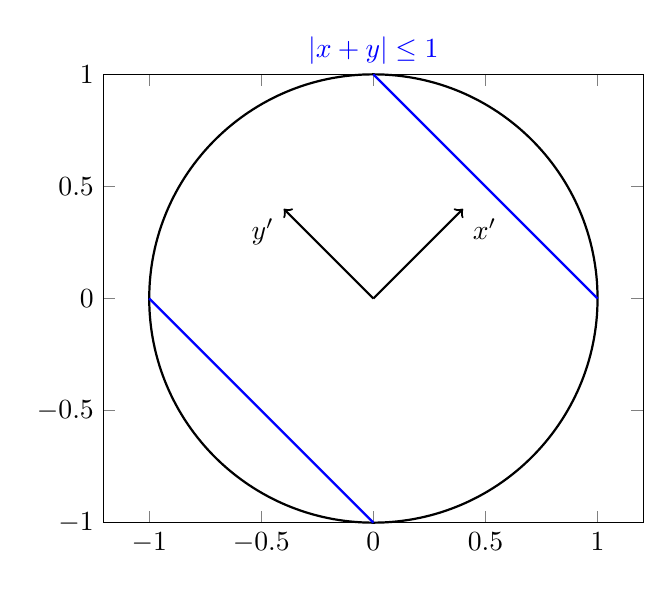
\begin{tikzpicture}
			\begin{axis}[xmin=-1,xmax=1,ymin=-1,ymax=1,axis equal,clip=false]
			\draw[thick] (axis cs: 0,0) circle (1);
			\addplot[domain=0:1,blue,thick] {1-x};
			\addplot[domain=-1:0,blue,thick] {-1-x};
			\draw (axis cs:0,1) node[anchor=south,blue] {$|x+y|\le 1$};
			\draw[thick,->] (axis cs:0,0) -- (axis cs:0.4,0.4);
			\draw[thick,->] (axis cs:0,0) -- (axis cs:-0.4,0.4);
			\draw (axis cs: 0.4,0.4) node[anchor=north west] {$x'$};
			\draw (axis cs:-0.4,0.4) node[anchor=north east] {$y'$};
			\end{axis}
		\end{tikzpicture}
	\end{center}
	Wir rotierenden dann das Koordinatensystem wie im Diagramm.
	\begin{center}
		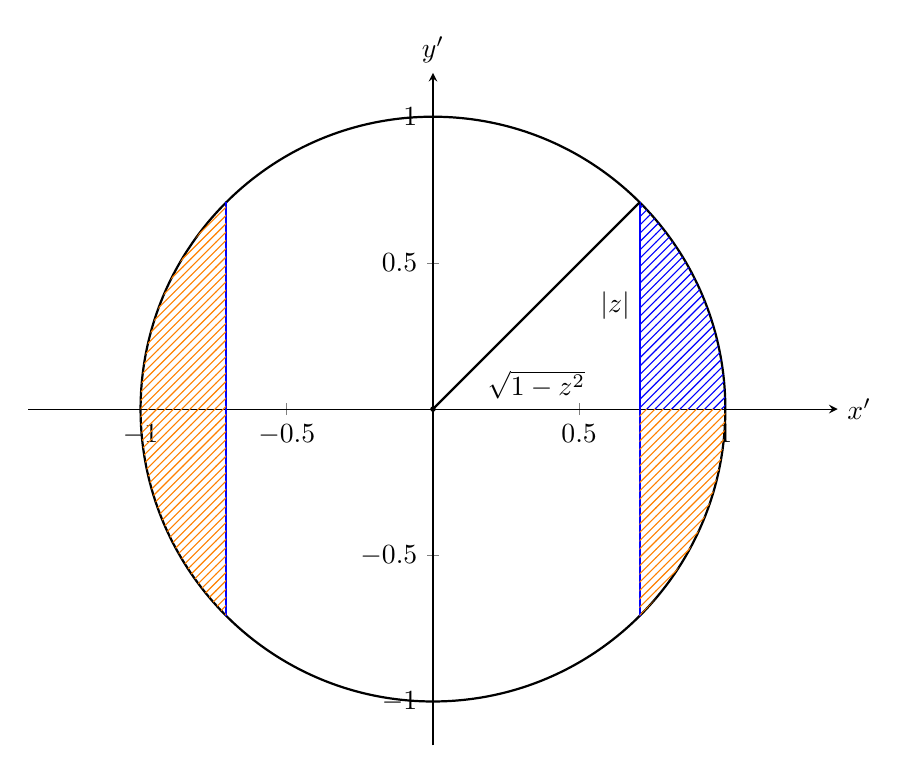
\begin{tikzpicture}
			\begin{axis}[xmin=-1.15,xmax=1.15,ymin=-1.15,ymax=1.15,xlabel=$x'$,ylabel=$y'$, axis equal,clip=false,axis lines = center, y label style={anchor=south}, x label style ={anchor=west},scale=1.5,xtick={-1,-0.5,0,0.5,1},ytick={-1,-0.5,0,0.5,1}]
				\draw[thick] (axis cs:0,0) circle (1);
				\draw[thick,blue] (axis cs:{1/sqrt(2)},{-1/sqrt(2)}) -- (axis cs:{1/sqrt(2)}, {1/sqrt(2)});
				\draw[thick,blue] (axis cs:{-1/sqrt(2)},{-1/sqrt(2)}) -- (axis cs:{-1/sqrt(2)}, {1/sqrt(2)});
			\fill (axis cs:0,0) circle (1pt);
				\draw[thick] (axis cs:0,0) -- (axis cs:{1/sqrt(2)},{1/sqrt(2)});
				\draw (axis cs:{1/sqrt(2)},{1/(2*sqrt(2))}) node[anchor=east] {$|z|$};
				\fill[pattern=north east lines,pattern color=blue] (axis cs:{1/sqrt(2)},{1/sqrt(2)}) arc(45:0:1) -- (axis cs:{1/sqrt(2)},0) -- cycle;
				\fill[pattern=north east lines,pattern color=orange] (axis cs:{1/sqrt(2)},{-1/sqrt(2)}) arc(-45:0:1) -- (axis cs:{1/sqrt(2)},0) -- cycle;
				\fill[pattern=north east lines, pattern color=orange] (axis cs:{-1/sqrt(2)},{1/sqrt(2)}) arc(135:225:1) -- cycle;
				\draw (axis cs:{1/(2*sqrt(2))},0) node[anchor=south] {$\sqrt{1-z^2} $};
			\end{axis}
		\end{tikzpicture}
	\end{center}
	Das Maß der blauen Region ist
	\[
		\frac{1}{2}\sin^{-1}|z|-\frac{1}{2}|z|\sqrt{1-z^2} 
	,\]
	also das Maß von $A_z$ ist
	\begin{align*}
		\lambda_2(A_z)=&\pi(1)^2-4\cdot\frac{1}{2}\left( \sin^{-1}|z|-|z|\sqrt{1-z^2}  \right)\\
		=&\pi-2\left( \sin^{-1}|z|-|z|\sqrt{1-z^2}  \right) 
	\end{align*}
	Dann ist
	\begin{align*}
		\lambda_3(A)=&\int_{-1}^1 \pi-2(\sin^{-1}|z|-|z|\sqrt{1-z^2} \dd{z}\\
		=&2\int_0^1 \pi-2(\sin^{-1}|z|-|z|\sqrt{1-z^2} \dd{z}\\
		=&2\int_0^1\pi-2(\sin^{-1}z-z\sqrt{1-z^2}) \dd{z}\\
		=&2\left[ \int_0^1 \pi\dd{z}-2\int_0^1\sin^{-1}z\dd{z}+2\int_0^1 z\sqrt{1-z^2} \dd{z} \right]\\
		=&2\left[ \pi-2\int_0^1 \sin^{-1}z\dd{z}+2\int_0^1 z\sqrt{1-z^2} \dd{z} \right]. 
	\end{align*}
	Nebenrechnung:
	\begin{align*}
		\int_0^1 \sin^{-1}z\dd{z}=&z\sin^{-1}z|_0^1-\int_0^1 \frac{z}{\sqrt{1-z^2} }\dd{z}\\
		=&\frac{\pi}{2}-\int_0^1 \frac{z}{\sqrt{1-z^2} }\dd{z}\\
		u=&1-z^2,\qquad \dd{u}=-2z\dd{z}\\
		\int_0^1\sin^{-1}z\dd{z}=&\frac{\pi}{2}+\frac{1}{2}\int_1^0 \frac{1}{\sqrt{u} }\dd{u}\\
		=&\frac{\pi}{2}+\sqrt{u}|_1^0\\
		=&\frac{\pi}{2}-1\\
		\int_0^1 z\sqrt{1-z^2} \dd{z}=&-\frac{1}{2}\int_1^0 \sqrt{u} \dd{u}\\
		=&\frac{1}{2}\int_0^1 \sqrt{u} \dd{u}\\
		=&\frac{1}{3}u^{3 / 2}|_0^1\\
		=&\frac{1}{3}
	\end{align*}
	Eingesetzt:
	\begin{align*}
		\lambda_3(A)=&2\left[ \pi-2\left( \frac{\pi}{2}-1 \right) +\frac{2}{3} \right] \\
		=&2\pi-4\left( \frac{\pi}{2}-1 \right) +\frac{4}{3}\\
		=&2\pi-2\pi+4+\frac{4}{3}\\
		=&\frac{16}{3}.\qedhere
	\end{align*}
\end{proof}
\begin{Problem}
	Sei $S\in \R^{n\times n}$ ein invertierbare Matrix und $a\in \R^n$. Definere damit die Abbildung $\varphi:\R^n\to \R^n, x\to a+Sx$. Sei außerdem $A\in \mathcal{L}(n)$ und $f:\R^n\to \R$ $\mathcal{L}(n)-B^1$ messbar, sodass $\chi_{\varphi(A)}f$ $\lambda_n$ integrierbar ist. Zeigen Sie, dass dann $\chi_A(f\circ \varphi)$ $\lambda_n$-integrierbar ist mit
	\[
		\int_{\varphi(A)}f\dd{\lambda_n}=|\text{det}(S)|\int_A (f\circ\varphi) \dd{\lambda_n}
	.\] 
	{\footnotesize \emph{Hinweis: Lemma 2.92}}
\end{Problem}
\begin{proof}
	Nach Satz 1.83 und Bewegungsinvarianz ist $\varphi(A)$ messbar mit Maß $\lambda_n(\varphi(A))=|\text{det}(S)|\lambda_n(A)$. $\chi_{\varphi(A)}$ ist dann messbar. Weil $\varphi$ affin ist, ist $\varphi$ stetig und daher messbar. Dann ist $f\circ\varphi$ messbar, und als Produkt von messbare Funktionen ist $\chi_A(f\circ \varphi)$ $\lambda_n$-messbar.

	Wir verwenden Lemma 2.93 und betrachten $f^+$. Es gilt
	\begin{align*}
		\int_{\varphi(A)}f^+\dd{\mu}=&\int f^+\chi_{\varphi(A)}\dd{\mu}\\
		=&\int_{(0,+\infty)}\mu(\{x:f^+(x)\chi_{\varphi}(A)>t\})\dd{\lambda_1(t)}\\
		=&\int_0^\infty \mu(\{x:x\in \varphi(A)\wedge f^+(x)>t\} \dd{\lambda_1(t)}\\
		=&\int_0^\infty\mu(\{x:f^+(x)>t\} \cap \varphi(A))\dd{\lambda_1(t)}
	\end{align*}
	Weil $\varphi$ bijektiv ist, gibt es f\"{u}r jedes Punkt  $x\in\varphi(A),~f^+(x)>t$ auch ein Punkt $y:=\varphi^{-1}(x),~y\in A,~f^+(\varphi(y))>t$ und andersherum. Daher ist 
	\[
	\{x:x\in \varphi(A)\wedge f^+(x)>t\} =\varphi(\{x:x\in A\wedge f^+(\varphi(x))>t\})
	.\] 
	Daraus folgt:
	\begin{align*}
		\int_{\varphi(A)}f^+\dd{\mu}=&\int_0^\infty \mu(\varphi(\{x:x\in A\wedge f^+(\varphi(x))>t\} ))\\
		=&\int_0^\infty|\text{det}(S)|\mu(\{x:x\in A\wedge f^+(\varphi(x))>t\})\dd{\lambda_1(t)}  \\
		&\text{(Satz 1.83 und Bewegungsinvarianz)}\\
		=&|\text{det}(S)|\int_0^\infty \mu(\{x:f^+(\varphi(x))>t\}\cap A)\\
		=&|\text{det}(S)|\int_0^\infty \mu(\{x:f^+(\varphi(x))\chi_A(x)>t\} )\dd{\lambda_1(t)}\\
		=&|\text{det}(S)|\int (f^+\circ\varphi)\chi_A\dd{\lambda_n}\\
		=&|\text{det}(S)|\int_A (f^+\circ\varphi)\dd{\lambda_n}
	\end{align*}
	Ähnlich gilt es auch für $-f^-$ und aus
	\[
	\int_{\varphi(A)}f\dd{\mu}=\int_{\varphi(A)} f^+\dd{\mu}-\int_{\varphi(A)}(-f^-)\dd{\mu}
	\]
	auch für $f$.
\end{proof}

\begin{Problem}
	Sei $f\in \mathcal{L}^1(\lambda_n)$. F\"{u}r $h\in \R^n$ definiere die Funktion $f_h:\R^n\to \R$ durch $f_h(x):=f(x+h)$. Definiere außerdem die Abbildung
	\[
	T_f:\R^n\to \mathcal{L}^1(\lambda_n),\qquad h\to f_h
	.\] 
	Zeigen Sie:
	\begin{parts}
		\item $T_f$ ist wohldefiniert.
		\item $T_f$ ist stetig.
	\end{parts}
{\footnotesize \emph{Hinweis: Approximieren Sie die Funktion }$f$ }
\end{Problem}

\begin{proof}
	\begin{parts}
	\item Hier zeigen wir: $f_h(x)\in \mathcal{L}^1(\lambda_n)$ f\"{u}r alle $h\in \R^n$. Wir brauchen zuerst: $f_h$ ist messbar. 
		\[
	\{f_h<\alpha\} =\{f<\alpha\} +h
,\]
		was messbar ist, was sonst ein Widerspruch zu der Bewegungsinvarianz wäre. Weil $(\R^n, \mathcal{L}(n), \lambda_n)$ $\sigma$-endlich ist, verwenden wir Satz 2.93:
		\begin{align*}
			\int |f|\dd{\lambda_n}=&\int_0^\infty \lambda_n(\{x:|f_h(x)|>t\})\dd{\lambda_1(t)}\\
			=&\int_0^\infty \lambda_n(\{x:|f(x)|>t\} +h)\dd{\lambda_1(t)}\\
			=&\int_0^\infty \lambda_n(\{x:|f(x)|>t\})\dd{\lambda_1(t)} & \text{Bewegungsinvarianz}\\
			=&\int |f|\dd{\lambda_n}<\infty & \text{Voraussetzung}
		\end{align*}
also $f_h\in \mathcal{L}^1(\lambda_n)$.
\item 
Nach Satz 2.101 gibt es eine stetige Funktion mit kompaktem Support $f_\epsilon$, so dass
	\[
		\|f-f_\epsilon\|_{\mathcal{L}^1(\mu)}<\epsilon
	.\] 
	Dann beweisen wir die Behauptung für stetige Funktionen mit kompaktem Träger, also sei $f$ eine solche Abbildung. Weil $f$ stetig auf einer kompakten Menge ist, ist $f$ gleichmäßig stetig. Sei $A$ der Träger von $f$. Sei $\epsilon>0$ gegeben. Dann gibt es ein $\delta<0$, so dass $|x-y|<\delta\implies |f(x)-f(y)|<\epsilon$. Daraus folgt:
	\[
		\|f-f_h\|_{\mathcal{L}^1(\lambda_n)}\le \int \epsilon\dd{\lambda_n}=\epsilon\lambda_n(A)
	.\] 
	Weil $A$ kompakt ist, hat $A$ endliches Maß. Die Behauptung folgt.

	Jetzt sind wir fertig, die Behauptung f\"{u}r beliebiges $f$ zu beweisen. Wir definieren außerdem $f_{\epsilon,h}=f_\epsilon(x+h)$, was auch messbar, stetig und mit kompaktem Support ist. Aus Bewegungsinvarianz gilt
\[
	\|f_h-f_{\epsilon,h}\|_{\mathcal{L}^1(\lambda_n)}=\|f-f_\epsilon\|_{\mathcal{L}^1(\lambda_n)}<\epsilon
.\] 
	Daraus folgt:
	\begin{align*}
		\|f-f_h\|_{\mathcal{L}^1(\lambda_n)}=&\|f-f_\epsilon+f_\epsilon-f_h\|_{\mathcal{L}^1(\lambda_n)}\\
		=&\|f-f_\epsilon\|_{\mathcal{L}^1(\lambda_n)}+\|f_\epsilon-f_h\|_{\mathcal{L}^1(\lambda_n)}\\
		\le&\epsilon + \|f_\epsilon-f_{\epsilon,h}+f_{\epsilon,h}-f_h\|_{\mathcal{L}^1(\lambda_n)}\\
		\le&\epsilon+\|f_\epsilon-f_{\epsilon,h}\|_{\mathcal{L}^1(\lambda_n)}+\|f_{\epsilon,h}-f_h\|_{\mathcal{L}^1(\lambda_n)}\\
		\le&2\epsilon+\|f_\epsilon-f_{\epsilon,h}\|_{\mathcal{L}^1(\lambda_n)}\\
		\le&3\epsilon\qquad |h|<\delta
	\end{align*}
	wobei im letzten Schritt wir die vorherigen Gezeigten benutzt haben, um $\delta$ hinreichend klein zu wählen, damit $\|f_\epsilon-f_{\epsilon,h}\|_{\mathcal{L}^1(\lambda_n)}<\epsilon$ f\"{u}r alle $|h|<\delta$.\qedhere
	\end{parts}
\end{proof}

%	\begin{Problem}
	Bestimmen Sie alle Isomorphietypen f\"{u}r Gruppen der Ordnung $45=3^2\cdot 5$.
\end{Problem}
\begin{proof}
	Wir betrachten die Zahl der $3$- bzw. $5$-Sylowgruppen $n_3$ bzw. $n_5$. Es gilt
	\begin{align*}
		n_3\equiv& 1\pmod{3}\\
		n_3|& 5\\
		n_5\equiv& 1\pmod{5}\\
		n_5|& 9
	\end{align*}
	Die einzige Lösung ist $n_3=1$ und $n_5=1$. Da die Zahlen $1$ sind, sind die Untergruppen normal. Sei $A$ die $3$-Sylowgruppe und $B$ die $5$-Sylowgruppe. Die Gruppen müssen sich trivial schneiden, weil die Ordnung alle Elemente darin ein Teiler von der Gruppenordnung sein müssen. 

	Da $9\times 5=45$, ist $|AB|=45$, also $AB$ ist einfach die ganze Gruppe. Da $n_3=n_5=1$, sind die Untergruppen normal. Es folgt daraus, dass die ganze Gruppe (isomorph zu) $A\times B$ ist.

	Also ist jetzt die Frage: Wie viele Gruppen der Ordnung $5$ und $9$ gibt es?

	Es gibt nur eine (bis auf Isomorphie) eindeutige Gruppe der Ordnung $5$, weil $5$ eine Primzahl ist, also es enthält ein Element der Ordnung $5$, was ein Erzeuger ist. Daher ist die Gruppe $C_5$.

	Wir wissen aus der vorherigen Übungsblatt, dass eine Gruppe der Ordnung $3^2$ abelsch ist. Dann ist eine Gruppe der Ordnung $9$ ein direktes Produkt von zyklische Gruppen von Primpotenzordnung. Die einzige Möglichkeit ist $C_3\times C_3$. Natürlich ist $C_9$ auch eine Gruppe der Ordnung $9$. 

	Insgesamt gibt es nur zwei Gruppen der Ordnung $45$: $C_5\times C_9$ und $C_5\times C_3\times C_3$.
\end{proof}
\begin{Problem}\label{pr:introalgblatt10-2}
	Seien $N$ und $U$ zwei Gruppen. Zeigen Sie: Genau dann gilt $N\rtimes_{\phi}U=N\times U$, wenn $\phi_u=\text{id}_N$ f\"{u}r alle $u\in U$ gilt.
\end{Problem}
\begin{proof}
	Die beide Gruppen sind auf der Menge $N\times U$ (kartesisches Produkt von Mengen) definiert. Jetzt die Rückrichtung: Falls $\phi_u=\text{id}_N$ f\"{u}r alle $N$ gilt, ist das Produkt
	\[
		(n_1,u_1)\circ (n_2,n_2)=(n_1\phi_{u_1}(n_2),u_1u_2)=(n_1n_2,u_1u_2)
	\]
	f\"{u}r alle $n_1,n_2\in N, u_1,u_2\in U$. Dann bekommen wir per Definition das direktes Produkt.

	Sei jetzt $N\rtimes_{\phi}U=N\times U$. Dann stimmen alle Produkte überein. Sei $u_1,u_2\in U$ und $n_1,n_2\in N$. Es gilt
	\[
		(n_1\phi_{u_1}(n_2),u_1u_2)=(n_1n_2,u_1u_2)
	\]
	insbesondere
	\[
		n_1\phi_{u_1}(n_2)=n_1n_2
	.\] 
	Aus der Kurzungsregel folgt
	\[
		\phi_{u_1}(n_2)=n_2
	.\] 
	Da $u_1,u_2,n_1,n_2$ beliebig waren, muss dies f\"{u}r alle $u_1,n_2$ gelten, also $\phi_{u_1}=\text{id}_N$ f\"{u}r alle $u_1\in U$.
\end{proof}
\begin{Problem}
	Von einer Gruppe $G$ seien bekannt:
	\begin{enumerate}[label=(\arabic*)]
		\item Sie habe Ordnung $p^2\cdot q^2$ mit zwei verschiedenen Primzahlen $p,q\in \mathbb{P}$.
		\item Die $q$-Sylowgruppe $Q$ von $G$ sei normal.
		\item $p$ Sei kein Teiler von $|\text{Aut}(Q)|$.
	\end{enumerate}
	Zeigen Sie, dass $G$ abelsch ist.

	(Hinweis: Denken Sie an semidirekte Produkte. Verwenden Sie an geeigneter Stelle Übung \ref{pr:introalgblatt10-2}.)  
\end{Problem}
\begin{proof}
	Sei die $p$-Sylowgruppe bzw. $q$-Sylowgruppe von $G$ $P$ bzw. $Q$. Es gilt $|P| |Q|=|G|$, also $G=PQ$. Da $Q$ normal ist, ist $G\cong Q\rtimes P$.  
\end{proof}
\begin{Problem}
	\begin{parts}
	\item Zeigen Sie, dass jede abelsche Gruppe der Ordnung $100$ ein Element der Ordnung $10$ enthält
	\item Zeigen Sie, dass $A_4$ keine Untergruppe der Ordnung $6$ besitzt (vgl. auch Bemerkung 2.29 im Skript).
	\end{parts}
\end{Problem}

%	\begin{Problem}
	\textbf{(Hyperbelfunktion)} Sei $d\in \{1,2,3\} , R>0, 1\le p<\infty$ und $\alpha>0$. Definiere
	\[
	B_R(d;0):=\{x\in \R^d|\|x\|<R\} , \qquad f:\R^d\to \R, x\to \begin{cases}
		0 & x=0,\\
		\frac{1}{\|x\|^\alpha} & x\neq 0.
	\end{cases}
	.\] 
	\begin{parts}
		\item Sei zunächst $d=1$. F\"{u}r welche $\alpha, p$ ist die Funktion $\chi_{B_R(1;0)}f$ in $L^p(\lambda_1)$? F\"{u}r welche $\alpha,p$ ist die Funktion $\chi_{\R\backslash B_R(1;0)}f$ in $L^p(\lambda_1)$?
		\item Welche Bedingungen müssen in den Fällen $d=2,3$ f\"{u}r $\alpha, p$ gelten, damit $\chi_{B_R(d;0)}f\in L^p(\lambda_d)$ ist?
		\item Sei $1<p<r<q<\infty$. Geben Sie eine Funktion $g:\R\to \R$ an mit $g\in L^r(\lambda_1)$, $g \not\in L^p(\lambda_1)$, $g \not\in L^q(\lambda_1)$.
		\item Geben Sie ein Beispiel f\"{u}r eine Funktion $g:(0,1)\to \R$ an, sodass $g\in L^p(\lambda_1)$ f\"{u}r alle $p\in [1,\infty)$ gilt, aber $g \not\in L^\infty(\lambda_1)$.
	\end{parts}
\end{Problem}

\begin{Problem}
	Sei $(X, \mathcal{A},\mu)$ ein Maßraum und $1\le p<q\le\infty$.
	\begin{parts}
	\item Zeigen Sie, dass $L^p(\mu)\cap L^q(\mu)\subseteq L^r(\mu)$ f\"{u}r alle $r\in (p,q)$ gilt und außerdem
		\[
			\|f\|_{L^r(\mu)}\le \|f\|_{L^p(\mu)}^\theta \|f\|_{L^q(\mu)}^{1-\theta}
		\] 
		f\"{u}r alle $f\in L^p(\mu)\cap L^q(\mu)$ und $\theta\in (0,1)$ mit
		\[
		\frac{1}{r}=\frac{\theta}{p}+\frac{1-\theta}{q}
		.\] 
	\item Sei der Maßraum $(X,\mathcal{A},\mu)$ nun endlich. Zeigen Sie, dass dan $L^q(\mu)\subseteq L^p(\mu)$ und
		\[
			\|f\|_{L^p(\mu)}\le \mu(X)^{\frac{1}{p}-\frac{1}{q}}\|f\|_{L^q(\mu)}
		\] 
		f\"{u}r alle $f\in L^q(\mu)$ gilt.

		\emph{Hinweis: Betrachten Sie den Raum $L^r(\mu)$ f\"{u}r $r:=\frac{q}{p}$.}
	\end{parts}
\end{Problem}

\begin{Problem}
	Sei $f:\R^3\to \R$ definiert durch $f(x,y,z):=|xyz|$ und
	\[
		A:=\left\{ (x,y,z)\in \R^3|x^2+y^2+z^2\le 1, z\ge \frac{1}{2} \right\} 
	.\] 
	Bestimmen Sie $\int_A f\dd{\lambda_3}$.
\end{Problem}

	\begin{Problem}
	Begründen Sie, warum die Determinante $\text{det}:\R^{n\times n}\to \R$ unendlich oft differenzierbar ist, und bestimmen Sie die Ableitung im Punkt $X\in \R^{n\times n}$. Welche besondere Form nimmt $(D\text{det})(\text{Id})$ an?  	
\end{Problem}
\begin{proof}
	Per Definition ist
	\[
		\text{det}(X)=\sum_{\sigma\in S_n} \text{sgn}(\sigma)X_{1\sigma(1)}X_{2\sigma(2)}\dots X_{n\sigma(n)}
	.\] 
	Da dies eine Summe von Produkte der Komponenten sind, ist $\text{det}$ unendlich oft differenzierbar.

	Es gilt $\text{det}':\R^{n\times n}\to\text{Hom}(\R^{n\times n},\R)$. Wir betrachten eine parameterabhängige Matrix $A(t)$. Es gilt
	\begin{align*}
	\dv{t}\text{det}A(t)=&\dv{t}\sum_{\sigma\in S_n}\text{sgn}(\sigma)A_{1\sigma(1)}(t)\dots A_{n\sigma(n)}(t)\\
		=&\sum_{\sigma\in S_n}\left[ (A_{1\sigma(1)}\dots A_{n\sigma(n)}) \sum_{j=1}^n\frac{A_{j\sigma(j)}'(t)}{A_{j\sigma(j)}} \right] \\
				=&\sum_{j=1}^n\sum_{\sigma\in S_n}\left[ (A_{1\sigma(1)}\dots A_{n\sigma(n)}) \frac{A_{j\sigma(j)}'(t)}{A_{j\sigma(j)}} \right] 
	\end{align*}
	F\"{u}r festes $j$ kann dieser Ausdruck so vorgestellt werden: Wir setzten in der $j$-te Zeile $A'$ statt $A$, also 
			\begin{center}
		\begin{tikzpicture}
			\matrix (M)[matrix of math nodes, row sep = 0.5cm, column sep = 0.5cm,left delimiter={(},right delimiter={)}]{
				A_{11}(t) & A_{12}(t) & \dots & A_{1n}(t)\\
				A_{21}(t) & A_{22}(t) & \dots & A_{2n}(t)\\
				\vdots & \vdots  & \ddots & \vdots\\
				A_{j1}'(t) & A_{j2}'(t) & \dots & A_{jn}'(t)\\
				\vdots & \vdots & \ddots & \vdots\\
				A_{n1}(t) & A_{n2}(t) & \dots & A_{nn}(t)\\
			};
			\draw[thick, blue] (-3.5,-0.5) -- (3.5,-0.5);
			\draw (3.6,-0.5) node[anchor=west,blue] {$j$-te Zeile};
		\end{tikzpicture}
	\end{center}
	und berechnen deren Determinante. Wir führen eine Laplaceentwicklung um die $j$-te Zeile durch und erhalten, mit $A^\#$ die adjugierte Matrix
	\begin{align*}
		\dv{t}\text{det} A(t)=&\sum_{j=1}^n\sum_{k=1}^n A_{jk}'(t)A^{\#}_{kj}\\
		=&\sum_{k=1}^n\sum_{j=1}^n A^{\#}_{kj}A_{jk}'(t)\\
		=&\sum_{k=1}^n (A^{\#} A')_{kk}\\
		=&\text{tr}(A^{\#}A')
	\end{align*}
	Also die Ableitung $\text{det}'$ im Punkt $A$ ist die Abbildung, die $B$ nach $\text{tr}(A^{\#}B)$ abbildet. 

	Im Punkt $I$: Es gilt $I^\#=I$, also $D\text{det}(I)=\text{tr}$.
\end{proof}
\begin{Problem}
	Ist $U\subset \R^n$ offen und $f:U\to \R$ zweimal differenzierbar, so kann die zweite Ableitung $D^2f$ in jedem Punkt $x\in U$ durch eine blineare Abbildung $\text{Hom}(\R^n,\R^n;\R)$ darstellen. F\"{u}r eine gegebene Basis auf dem $\R^n$-wir wählen die kanonische Basis hier - lassen sich bilineare Abbildungen durch eine Matrix $A\in \R^{n\times n}$ darstellen, die sog. Hesse-Matrix $Hf$ mit
	\[
		Hf(x,y)=\left[ \pdv[2]{f}{x_i}{x_j}(x) \right]_{i,j=1,\dots, n}=\begin{pmatrix} \pdv[2]{f}{x_1}{x_1} & \dots & \pdv[2]{f}{x_1}{x_n} \\ \vdots & \ddots & \vdots \\ \pdv[2]{f}{x_1}{x_n} & \dots & \pdv[2]{f}{x_n}{x_n}\end{pmatrix} 
	.\] 
Hier wurde schon ausgenutzt, dass die partiellen Ableitungen nach dem Satz von Schwarz vertauschen, die Hesse-Matrix ist also symmetrisch.

Es sei nun $f:\R^n\to \R$ mit
\[
	f(x)=\frac{1}{2}x^T Ax=\frac{1}{2}\sum_{i,j=1}^n a_{ij}x_i x_j
\]
f\"{u}r eine Matrix $A\in \R^{n\times n}$.
\begin{parts}
	\item Zeigen Sie, dass $f$ in $(0,0)$ ein Minimum, Maximum oder Sattelpunkt genau dann besitzt, wenn die Hesse-Matrix von $f$ (in (0,0)) positiv semi- negativ semi- bzw. indefinit ist. 
	\item Zeigen Sie durch ein Beispiel, dass für allgemeine Funktionen mit positiv (bzw. negativ) semidefiniter Hesse-Matrix im kritischen Punkt kein lokales Minimum (bzw. Maximum) vorliegen muss.  
\end{parts}
\end{Problem}
\begin{proof}
	\begin{parts}
	\item Offensichtlich ist $A$ die Hesse-Matrix und $f(0)=0$. Wir drücken $f(x)$ als $\frac{1}{2}\langle x, Ax\rangle$ aus.

	Dann per Definition: Falls $A$ positiv semidefinit ist, ist $f(x)=\frac{1}{2}\langle x, Ax\rangle\ge 0$ f\"{u}r alle $x$, also $f$ besitzt ein Minimum in $(0,0)$. Die Umkehrrichtung gilt auch per Definition. Sei $U$ eine Umgebung. F\"{u}r $x\in U$ ist $\langle x, Ax\rangle \ge 0$ per Definition eines Minimums. 

	Das gleiche Argument (per Definition) gilt f\"{u}r $f$ ein Maximum in $(0,0)$.
\item Die Funktion $f:\R\to\R$ mit $f(x)=x^3$ besitzt in $0$ Ableitung $0$. $0$ ist sowohl positiv als auch negativ definit. Die Funktion besitzt aber weder ein Maximum noch ein Minimum in $0$.
\end{parts}
\end{proof}
\begin{Problem}
	Es sei
	\[
		F:\R^2\to \R^2, \qquad F(x,y)=(x^2-y^2,2xy)^T
	.\] 
	\begin{parts}
	\item Berechnen Sie die Jacobi-Matrix von $F$.
	\item In welchem Punkt $p\in \R^2$ existiert die Inverse von $JF(p)$?
	\item Finden Sie eine lokale inverse Abbildung $F^{-1}$ von $F$ in einer Umgebung von $p=(1,0)=F(1,0)$ und berechnen Sie die Ableitung von $F^{-1}$ in $p$.
	\item Ist $F$ auf dem ganzen Gebiet $\{p\in \R^2|JF(p)\text{ invertierbar}\} $ global invertierbar?
	\end{parts}
\end{Problem}
\begin{proof}
	\begin{parts}
	\item
		\[
			JF=\begin{pmatrix} 2x & -2y \\ 2y & 2x \end{pmatrix} 
		.\] 
	\item $\text{det}(JF)=4x^2+4y^2$. Dies ist genau dann Null, wenn $x=y=0$. Sonst ist $JF$ invertierbar.
	\item Wir lösen das Gleichungssystem:
		\begin{align*}
			x^2-y^2=&\xi\\
			2xy=&\zeta\\
			y=&\frac{\zeta}{2x}\\
			x^2-\left( \frac{\zeta}{2x} \right)^2=&\xi\\
			x^4-\frac{\zeta^2}{4}=&\xi x^2\\
			x^4 - \xi x^2-\frac{\zeta^2}{4}=&0\\
			x^2=\frac{1}{2}\left[ \xi\pm \sqrt{\xi^2+\zeta^2}  \right] 
		\end{align*}
		Beim Punkt $(x,y)=(1,0)$ ist $(\xi,\zeta)=(1,0)$. In einer genug kleinen Umgebung nehmen wir daher die positive Nullstelle und danach positive Würzel.
		\[
			x=\left[ \frac{\xi+\sqrt{\xi^2+\zeta^2} }{2} \right]^{1 / 2}
		.\] 
		Daraus folgt:
		\[
			y=\frac{\zeta}{2}\left[ \frac{2}{\xi+\sqrt{\xi^2+\zeta^2} } \right]^{1 / 2}
		.\] 
		Dies ist die Umkehrabbildung.	
	\item Nein, weil sie nicht injektiv ist. Es gilt $F(1,1)=(0,2)$ und $F(-1,-1)=(0,2)$, aber $(1,1)\neq (-1,-1)$.\qedhere 
	\end{parts}
\end{proof}
\begin{Problem}
	Mithilfe des Satzes über implizite Funktionen beweisen wir die Glattheit der Inversen-Abbildung $\text{inf}:GL(n)\to GL(n)$. Gehen Sie wie folgt vor:
	\begin{parts}
	\item Begründen Sie, dass die Abbildung $A\cdot B\to AB$ auf $\R^{(n\times n)^2}$ unendlich oft differenzierbar ist.
	\item Nutzen Sie dan Satz über implizite Funktionen, um $\text{inf}\in \mathcal{C}^\infty (GL(n),GL(n))$ zu beweisen.

		\emph{Hinweis: Betrachten Sie $A\cdot B=\text{Id}$ }
	\end{parts}
\end{Problem}

\end{document}
